\documentclass[10pt,a4paper,oneside,onecolumn]{article}
% PACKAGES
\usepackage[utf8]{inputenc}
\usepackage[english]{babel}
\usepackage{pgf, pgfplots, tikz, booktabs, graphicx}
\usepackage{bookman}
%\usepackage[bitstream-charter]{mathdesign}
\usepackage[T1]{fontenc}
% SETTINGS
\author{Ludovic.Charleux@univ-usmb.fr}
\title{Scientific plotter benchmark}
\date{2015}

\newcommand{\blabla}[1] %Une commande pour remplir le vide
  {
  \foreach \n in {0,...,#1}{Lorem ipsum dolor sit amet, consectetur adipiscing elit, sed do eiusmod tempor incididunt ut labore et dolore magna aliqua. Ut enim ad minim veniam, quis nostrud exercitation ullamco laboris nisi ut aliquip ex ea commodo consequat. Duis aute irure dolor in reprehenderit in voluptate velit esse cillum dolore eu fugiat nulla pariatur. Excepteur sint occaecat cupidatat non proident, sunt in culpa qui officia deserunt mollit anim id est laborum. \\}
  }

\begin{document}
\maketitle
\tableofcontents
\newpage

\section{Simple Plot}

The goal is to plot data.csv in a 90 mm x 65 mm plot as follows.

\section{Raccoon Master : $\pi$thon }

\subsection{Matplotlib + PDF backend}
\blabla{1}
\begin{center}
\includegraphics{simple_plot/mpl.pdf}
\end{center}
\blabla{1}

\subsection{Matplotlib + PGF backend}
\blabla{1}
\begin{center}
%% Creator: Matplotlib, PGF backend
%%
%% To include the figure in your LaTeX document, write
%%   \input{<filename>.pgf}
%%
%% Make sure the required packages are loaded in your preamble
%%   \usepackage{pgf}
%%
%% Figures using additional raster images can only be included by \input if
%% they are in the same directory as the main LaTeX file. For loading figures
%% from other directories you can use the `import` package
%%   \usepackage{import}
%% and then include the figures with
%%   \import{<path to file>}{<filename>.pgf}
%%
%% Matplotlib used the following preamble
%%   \usepackage{fontspec}
%%   \setmonofont{Courier}
%%
\begingroup%
\makeatletter%
\begin{pgfpicture}%
\pgfpathrectangle{\pgfpointorigin}{\pgfqpoint{3.543309in}{2.530935in}}%
\pgfusepath{use as bounding box, clip}%
\begin{pgfscope}%
\pgfsetbuttcap%
\pgfsetmiterjoin%
\definecolor{currentfill}{rgb}{1.000000,1.000000,1.000000}%
\pgfsetfillcolor{currentfill}%
\pgfsetlinewidth{0.000000pt}%
\definecolor{currentstroke}{rgb}{1.000000,1.000000,1.000000}%
\pgfsetstrokecolor{currentstroke}%
\pgfsetdash{}{0pt}%
\pgfpathmoveto{\pgfqpoint{0.000000in}{0.000000in}}%
\pgfpathlineto{\pgfqpoint{3.543309in}{0.000000in}}%
\pgfpathlineto{\pgfqpoint{3.543309in}{2.530935in}}%
\pgfpathlineto{\pgfqpoint{0.000000in}{2.530935in}}%
\pgfpathclose%
\pgfusepath{fill}%
\end{pgfscope}%
\begin{pgfscope}%
\pgfsetbuttcap%
\pgfsetmiterjoin%
\definecolor{currentfill}{rgb}{1.000000,1.000000,1.000000}%
\pgfsetfillcolor{currentfill}%
\pgfsetlinewidth{0.000000pt}%
\definecolor{currentstroke}{rgb}{0.000000,0.000000,0.000000}%
\pgfsetstrokecolor{currentstroke}%
\pgfsetstrokeopacity{0.000000}%
\pgfsetdash{}{0pt}%
\pgfpathmoveto{\pgfqpoint{0.750465in}{0.572889in}}%
\pgfpathlineto{\pgfqpoint{3.302205in}{0.572889in}}%
\pgfpathlineto{\pgfqpoint{3.302205in}{2.169652in}}%
\pgfpathlineto{\pgfqpoint{0.750465in}{2.169652in}}%
\pgfpathclose%
\pgfusepath{fill}%
\end{pgfscope}%
\begin{pgfscope}%
\pgfpathrectangle{\pgfqpoint{0.750465in}{0.572889in}}{\pgfqpoint{2.551741in}{1.596763in}} %
\pgfusepath{clip}%
\pgfsetrectcap%
\pgfsetroundjoin%
\pgfsetlinewidth{1.003750pt}%
\definecolor{currentstroke}{rgb}{0.000000,0.000000,1.000000}%
\pgfsetstrokecolor{currentstroke}%
\pgfsetdash{}{0pt}%
\pgfpathmoveto{\pgfqpoint{0.750465in}{1.257216in}}%
\pgfpathlineto{\pgfqpoint{0.776240in}{1.328827in}}%
\pgfpathlineto{\pgfqpoint{0.802015in}{1.398713in}}%
\pgfpathlineto{\pgfqpoint{0.827790in}{1.466623in}}%
\pgfpathlineto{\pgfqpoint{0.853565in}{1.532319in}}%
\pgfpathlineto{\pgfqpoint{0.879341in}{1.595576in}}%
\pgfpathlineto{\pgfqpoint{0.905116in}{1.656186in}}%
\pgfpathlineto{\pgfqpoint{0.930891in}{1.713953in}}%
\pgfpathlineto{\pgfqpoint{0.956666in}{1.768697in}}%
\pgfpathlineto{\pgfqpoint{0.982441in}{1.820257in}}%
\pgfpathlineto{\pgfqpoint{1.008216in}{1.868484in}}%
\pgfpathlineto{\pgfqpoint{1.033991in}{1.913248in}}%
\pgfpathlineto{\pgfqpoint{1.059767in}{1.954435in}}%
\pgfpathlineto{\pgfqpoint{1.085542in}{1.991949in}}%
\pgfpathlineto{\pgfqpoint{1.111317in}{2.025710in}}%
\pgfpathlineto{\pgfqpoint{1.137092in}{2.055655in}}%
\pgfpathlineto{\pgfqpoint{1.162867in}{2.081737in}}%
\pgfpathlineto{\pgfqpoint{1.188642in}{2.103928in}}%
\pgfpathlineto{\pgfqpoint{1.214418in}{2.122215in}}%
\pgfpathlineto{\pgfqpoint{1.240193in}{2.136600in}}%
\pgfpathlineto{\pgfqpoint{1.265968in}{2.147103in}}%
\pgfpathlineto{\pgfqpoint{1.291743in}{2.153759in}}%
\pgfpathlineto{\pgfqpoint{1.317518in}{2.156618in}}%
\pgfpathlineto{\pgfqpoint{1.343293in}{2.155744in}}%
\pgfpathlineto{\pgfqpoint{1.369069in}{2.151214in}}%
\pgfpathlineto{\pgfqpoint{1.394844in}{2.143121in}}%
\pgfpathlineto{\pgfqpoint{1.420619in}{2.131570in}}%
\pgfpathlineto{\pgfqpoint{1.446394in}{2.116675in}}%
\pgfpathlineto{\pgfqpoint{1.472169in}{2.098566in}}%
\pgfpathlineto{\pgfqpoint{1.497944in}{2.077380in}}%
\pgfpathlineto{\pgfqpoint{1.523719in}{2.053266in}}%
\pgfpathlineto{\pgfqpoint{1.549495in}{2.026380in}}%
\pgfpathlineto{\pgfqpoint{1.575270in}{1.996888in}}%
\pgfpathlineto{\pgfqpoint{1.601045in}{1.964963in}}%
\pgfpathlineto{\pgfqpoint{1.626820in}{1.930784in}}%
\pgfpathlineto{\pgfqpoint{1.652595in}{1.894535in}}%
\pgfpathlineto{\pgfqpoint{1.678370in}{1.856407in}}%
\pgfpathlineto{\pgfqpoint{1.704146in}{1.816591in}}%
\pgfpathlineto{\pgfqpoint{1.729921in}{1.775286in}}%
\pgfpathlineto{\pgfqpoint{1.755696in}{1.732690in}}%
\pgfpathlineto{\pgfqpoint{1.781471in}{1.689002in}}%
\pgfpathlineto{\pgfqpoint{1.807246in}{1.644423in}}%
\pgfpathlineto{\pgfqpoint{1.833021in}{1.599153in}}%
\pgfpathlineto{\pgfqpoint{1.858796in}{1.553391in}}%
\pgfpathlineto{\pgfqpoint{1.884572in}{1.507334in}}%
\pgfpathlineto{\pgfqpoint{1.910347in}{1.461175in}}%
\pgfpathlineto{\pgfqpoint{1.936122in}{1.415106in}}%
\pgfpathlineto{\pgfqpoint{1.961897in}{1.369313in}}%
\pgfpathlineto{\pgfqpoint{1.987672in}{1.323977in}}%
\pgfpathlineto{\pgfqpoint{2.013447in}{1.279276in}}%
\pgfpathlineto{\pgfqpoint{2.039223in}{1.235378in}}%
\pgfpathlineto{\pgfqpoint{2.064998in}{1.192447in}}%
\pgfpathlineto{\pgfqpoint{2.090773in}{1.150640in}}%
\pgfpathlineto{\pgfqpoint{2.116548in}{1.110105in}}%
\pgfpathlineto{\pgfqpoint{2.142323in}{1.070981in}}%
\pgfpathlineto{\pgfqpoint{2.168098in}{1.033401in}}%
\pgfpathlineto{\pgfqpoint{2.193874in}{0.997487in}}%
\pgfpathlineto{\pgfqpoint{2.219649in}{0.963353in}}%
\pgfpathlineto{\pgfqpoint{2.245424in}{0.931103in}}%
\pgfpathlineto{\pgfqpoint{2.271199in}{0.900831in}}%
\pgfpathlineto{\pgfqpoint{2.296974in}{0.872621in}}%
\pgfpathlineto{\pgfqpoint{2.322749in}{0.846547in}}%
\pgfpathlineto{\pgfqpoint{2.348524in}{0.822673in}}%
\pgfpathlineto{\pgfqpoint{2.374300in}{0.801052in}}%
\pgfpathlineto{\pgfqpoint{2.400075in}{0.781728in}}%
\pgfpathlineto{\pgfqpoint{2.425850in}{0.764734in}}%
\pgfpathlineto{\pgfqpoint{2.451625in}{0.750093in}}%
\pgfpathlineto{\pgfqpoint{2.477400in}{0.737817in}}%
\pgfpathlineto{\pgfqpoint{2.503175in}{0.727910in}}%
\pgfpathlineto{\pgfqpoint{2.528951in}{0.720364in}}%
\pgfpathlineto{\pgfqpoint{2.554726in}{0.715163in}}%
\pgfpathlineto{\pgfqpoint{2.580501in}{0.712282in}}%
\pgfpathlineto{\pgfqpoint{2.606276in}{0.711686in}}%
\pgfpathlineto{\pgfqpoint{2.632051in}{0.713331in}}%
\pgfpathlineto{\pgfqpoint{2.657826in}{0.717167in}}%
\pgfpathlineto{\pgfqpoint{2.683602in}{0.723132in}}%
\pgfpathlineto{\pgfqpoint{2.709377in}{0.731162in}}%
\pgfpathlineto{\pgfqpoint{2.735152in}{0.741181in}}%
\pgfpathlineto{\pgfqpoint{2.760927in}{0.753109in}}%
\pgfpathlineto{\pgfqpoint{2.786702in}{0.766858in}}%
\pgfpathlineto{\pgfqpoint{2.812477in}{0.782337in}}%
\pgfpathlineto{\pgfqpoint{2.838252in}{0.799447in}}%
\pgfpathlineto{\pgfqpoint{2.864028in}{0.818086in}}%
\pgfpathlineto{\pgfqpoint{2.889803in}{0.838147in}}%
\pgfpathlineto{\pgfqpoint{2.915578in}{0.859520in}}%
\pgfpathlineto{\pgfqpoint{2.941353in}{0.882090in}}%
\pgfpathlineto{\pgfqpoint{2.967128in}{0.905743in}}%
\pgfpathlineto{\pgfqpoint{2.992903in}{0.930358in}}%
\pgfpathlineto{\pgfqpoint{3.018679in}{0.955818in}}%
\pgfpathlineto{\pgfqpoint{3.044454in}{0.982000in}}%
\pgfpathlineto{\pgfqpoint{3.070229in}{1.008784in}}%
\pgfpathlineto{\pgfqpoint{3.096004in}{1.036047in}}%
\pgfpathlineto{\pgfqpoint{3.121779in}{1.063669in}}%
\pgfpathlineto{\pgfqpoint{3.147554in}{1.091529in}}%
\pgfpathlineto{\pgfqpoint{3.173330in}{1.119510in}}%
\pgfpathlineto{\pgfqpoint{3.199105in}{1.147494in}}%
\pgfpathlineto{\pgfqpoint{3.224880in}{1.175366in}}%
\pgfpathlineto{\pgfqpoint{3.250655in}{1.203016in}}%
\pgfpathlineto{\pgfqpoint{3.276430in}{1.230334in}}%
\pgfpathlineto{\pgfqpoint{3.302205in}{1.257216in}}%
\pgfusepath{stroke}%
\end{pgfscope}%
\begin{pgfscope}%
\pgfpathrectangle{\pgfqpoint{0.750465in}{0.572889in}}{\pgfqpoint{2.551741in}{1.596763in}} %
\pgfusepath{clip}%
\pgfsetrectcap%
\pgfsetroundjoin%
\pgfsetlinewidth{1.003750pt}%
\definecolor{currentstroke}{rgb}{0.000000,0.500000,0.000000}%
\pgfsetstrokecolor{currentstroke}%
\pgfsetdash{}{0pt}%
\pgfpathmoveto{\pgfqpoint{0.750465in}{1.257216in}}%
\pgfpathlineto{\pgfqpoint{0.776240in}{1.327964in}}%
\pgfpathlineto{\pgfqpoint{0.802015in}{1.394767in}}%
\pgfpathlineto{\pgfqpoint{0.827790in}{1.456701in}}%
\pgfpathlineto{\pgfqpoint{0.853565in}{1.512957in}}%
\pgfpathlineto{\pgfqpoint{0.879341in}{1.562850in}}%
\pgfpathlineto{\pgfqpoint{0.905116in}{1.605826in}}%
\pgfpathlineto{\pgfqpoint{0.930891in}{1.641463in}}%
\pgfpathlineto{\pgfqpoint{0.956666in}{1.669477in}}%
\pgfpathlineto{\pgfqpoint{0.982441in}{1.689715in}}%
\pgfpathlineto{\pgfqpoint{1.008216in}{1.702160in}}%
\pgfpathlineto{\pgfqpoint{1.033991in}{1.706917in}}%
\pgfpathlineto{\pgfqpoint{1.059767in}{1.704215in}}%
\pgfpathlineto{\pgfqpoint{1.085542in}{1.694393in}}%
\pgfpathlineto{\pgfqpoint{1.111317in}{1.677891in}}%
\pgfpathlineto{\pgfqpoint{1.137092in}{1.655241in}}%
\pgfpathlineto{\pgfqpoint{1.162867in}{1.627052in}}%
\pgfpathlineto{\pgfqpoint{1.188642in}{1.594000in}}%
\pgfpathlineto{\pgfqpoint{1.214418in}{1.556811in}}%
\pgfpathlineto{\pgfqpoint{1.240193in}{1.516251in}}%
\pgfpathlineto{\pgfqpoint{1.265968in}{1.473109in}}%
\pgfpathlineto{\pgfqpoint{1.291743in}{1.428185in}}%
\pgfpathlineto{\pgfqpoint{1.317518in}{1.382275in}}%
\pgfpathlineto{\pgfqpoint{1.343293in}{1.336161in}}%
\pgfpathlineto{\pgfqpoint{1.369069in}{1.290597in}}%
\pgfpathlineto{\pgfqpoint{1.394844in}{1.246297in}}%
\pgfpathlineto{\pgfqpoint{1.420619in}{1.203928in}}%
\pgfpathlineto{\pgfqpoint{1.446394in}{1.164098in}}%
\pgfpathlineto{\pgfqpoint{1.472169in}{1.127352in}}%
\pgfpathlineto{\pgfqpoint{1.497944in}{1.094160in}}%
\pgfpathlineto{\pgfqpoint{1.523719in}{1.064918in}}%
\pgfpathlineto{\pgfqpoint{1.549495in}{1.039944in}}%
\pgfpathlineto{\pgfqpoint{1.575270in}{1.019472in}}%
\pgfpathlineto{\pgfqpoint{1.601045in}{1.003654in}}%
\pgfpathlineto{\pgfqpoint{1.626820in}{0.992563in}}%
\pgfpathlineto{\pgfqpoint{1.652595in}{0.986190in}}%
\pgfpathlineto{\pgfqpoint{1.678370in}{0.984451in}}%
\pgfpathlineto{\pgfqpoint{1.704146in}{0.987191in}}%
\pgfpathlineto{\pgfqpoint{1.729921in}{0.994189in}}%
\pgfpathlineto{\pgfqpoint{1.755696in}{1.005162in}}%
\pgfpathlineto{\pgfqpoint{1.781471in}{1.019776in}}%
\pgfpathlineto{\pgfqpoint{1.807246in}{1.037651in}}%
\pgfpathlineto{\pgfqpoint{1.833021in}{1.058368in}}%
\pgfpathlineto{\pgfqpoint{1.858796in}{1.081479in}}%
\pgfpathlineto{\pgfqpoint{1.884572in}{1.106517in}}%
\pgfpathlineto{\pgfqpoint{1.910347in}{1.133000in}}%
\pgfpathlineto{\pgfqpoint{1.936122in}{1.160442in}}%
\pgfpathlineto{\pgfqpoint{1.961897in}{1.188363in}}%
\pgfpathlineto{\pgfqpoint{1.987672in}{1.216291in}}%
\pgfpathlineto{\pgfqpoint{2.013447in}{1.243775in}}%
\pgfpathlineto{\pgfqpoint{2.039223in}{1.270388in}}%
\pgfpathlineto{\pgfqpoint{2.064998in}{1.295734in}}%
\pgfpathlineto{\pgfqpoint{2.090773in}{1.319454in}}%
\pgfpathlineto{\pgfqpoint{2.116548in}{1.341228in}}%
\pgfpathlineto{\pgfqpoint{2.142323in}{1.360782in}}%
\pgfpathlineto{\pgfqpoint{2.168098in}{1.377886in}}%
\pgfpathlineto{\pgfqpoint{2.193874in}{1.392363in}}%
\pgfpathlineto{\pgfqpoint{2.219649in}{1.404081in}}%
\pgfpathlineto{\pgfqpoint{2.245424in}{1.412960in}}%
\pgfpathlineto{\pgfqpoint{2.271199in}{1.418970in}}%
\pgfpathlineto{\pgfqpoint{2.296974in}{1.422126in}}%
\pgfpathlineto{\pgfqpoint{2.322749in}{1.422491in}}%
\pgfpathlineto{\pgfqpoint{2.348524in}{1.420169in}}%
\pgfpathlineto{\pgfqpoint{2.374300in}{1.415305in}}%
\pgfpathlineto{\pgfqpoint{2.400075in}{1.408077in}}%
\pgfpathlineto{\pgfqpoint{2.425850in}{1.398696in}}%
\pgfpathlineto{\pgfqpoint{2.451625in}{1.387399in}}%
\pgfpathlineto{\pgfqpoint{2.477400in}{1.374444in}}%
\pgfpathlineto{\pgfqpoint{2.503175in}{1.360107in}}%
\pgfpathlineto{\pgfqpoint{2.528951in}{1.344675in}}%
\pgfpathlineto{\pgfqpoint{2.554726in}{1.328439in}}%
\pgfpathlineto{\pgfqpoint{2.580501in}{1.311694in}}%
\pgfpathlineto{\pgfqpoint{2.606276in}{1.294732in}}%
\pgfpathlineto{\pgfqpoint{2.632051in}{1.277835in}}%
\pgfpathlineto{\pgfqpoint{2.657826in}{1.261274in}}%
\pgfpathlineto{\pgfqpoint{2.683602in}{1.245302in}}%
\pgfpathlineto{\pgfqpoint{2.709377in}{1.230156in}}%
\pgfpathlineto{\pgfqpoint{2.735152in}{1.216047in}}%
\pgfpathlineto{\pgfqpoint{2.760927in}{1.203163in}}%
\pgfpathlineto{\pgfqpoint{2.786702in}{1.191663in}}%
\pgfpathlineto{\pgfqpoint{2.812477in}{1.181678in}}%
\pgfpathlineto{\pgfqpoint{2.838252in}{1.173309in}}%
\pgfpathlineto{\pgfqpoint{2.864028in}{1.166629in}}%
\pgfpathlineto{\pgfqpoint{2.889803in}{1.161678in}}%
\pgfpathlineto{\pgfqpoint{2.915578in}{1.158468in}}%
\pgfpathlineto{\pgfqpoint{2.941353in}{1.156981in}}%
\pgfpathlineto{\pgfqpoint{2.967128in}{1.157174in}}%
\pgfpathlineto{\pgfqpoint{2.992903in}{1.158977in}}%
\pgfpathlineto{\pgfqpoint{3.018679in}{1.162297in}}%
\pgfpathlineto{\pgfqpoint{3.044454in}{1.167020in}}%
\pgfpathlineto{\pgfqpoint{3.070229in}{1.173014in}}%
\pgfpathlineto{\pgfqpoint{3.096004in}{1.180133in}}%
\pgfpathlineto{\pgfqpoint{3.121779in}{1.188215in}}%
\pgfpathlineto{\pgfqpoint{3.147554in}{1.197094in}}%
\pgfpathlineto{\pgfqpoint{3.173330in}{1.206593in}}%
\pgfpathlineto{\pgfqpoint{3.199105in}{1.216534in}}%
\pgfpathlineto{\pgfqpoint{3.224880in}{1.226740in}}%
\pgfpathlineto{\pgfqpoint{3.250655in}{1.237034in}}%
\pgfpathlineto{\pgfqpoint{3.276430in}{1.247246in}}%
\pgfpathlineto{\pgfqpoint{3.302205in}{1.257216in}}%
\pgfusepath{stroke}%
\end{pgfscope}%
\begin{pgfscope}%
\pgfsetrectcap%
\pgfsetmiterjoin%
\pgfsetlinewidth{1.505625pt}%
\definecolor{currentstroke}{rgb}{0.000000,0.000000,0.000000}%
\pgfsetstrokecolor{currentstroke}%
\pgfsetdash{}{0pt}%
\pgfpathmoveto{\pgfqpoint{0.750465in}{2.169652in}}%
\pgfpathlineto{\pgfqpoint{3.302205in}{2.169652in}}%
\pgfusepath{stroke}%
\end{pgfscope}%
\begin{pgfscope}%
\pgfsetrectcap%
\pgfsetmiterjoin%
\pgfsetlinewidth{1.505625pt}%
\definecolor{currentstroke}{rgb}{0.000000,0.000000,0.000000}%
\pgfsetstrokecolor{currentstroke}%
\pgfsetdash{}{0pt}%
\pgfpathmoveto{\pgfqpoint{3.302205in}{0.572889in}}%
\pgfpathlineto{\pgfqpoint{3.302205in}{2.169652in}}%
\pgfusepath{stroke}%
\end{pgfscope}%
\begin{pgfscope}%
\pgfsetrectcap%
\pgfsetmiterjoin%
\pgfsetlinewidth{1.505625pt}%
\definecolor{currentstroke}{rgb}{0.000000,0.000000,0.000000}%
\pgfsetstrokecolor{currentstroke}%
\pgfsetdash{}{0pt}%
\pgfpathmoveto{\pgfqpoint{0.750465in}{0.572889in}}%
\pgfpathlineto{\pgfqpoint{3.302205in}{0.572889in}}%
\pgfusepath{stroke}%
\end{pgfscope}%
\begin{pgfscope}%
\pgfsetrectcap%
\pgfsetmiterjoin%
\pgfsetlinewidth{1.505625pt}%
\definecolor{currentstroke}{rgb}{0.000000,0.000000,0.000000}%
\pgfsetstrokecolor{currentstroke}%
\pgfsetdash{}{0pt}%
\pgfpathmoveto{\pgfqpoint{0.750465in}{0.572889in}}%
\pgfpathlineto{\pgfqpoint{0.750465in}{2.169652in}}%
\pgfusepath{stroke}%
\end{pgfscope}%
\begin{pgfscope}%
\pgfpathrectangle{\pgfqpoint{0.750465in}{0.572889in}}{\pgfqpoint{2.551741in}{1.596763in}} %
\pgfusepath{clip}%
\pgfsetbuttcap%
\pgfsetroundjoin%
\pgfsetlinewidth{0.501875pt}%
\definecolor{currentstroke}{rgb}{0.000000,0.000000,0.000000}%
\pgfsetstrokecolor{currentstroke}%
\pgfsetdash{{1.000000pt}{3.000000pt}}{0.000000pt}%
\pgfpathmoveto{\pgfqpoint{0.750465in}{0.572889in}}%
\pgfpathlineto{\pgfqpoint{0.750465in}{2.169652in}}%
\pgfusepath{stroke}%
\end{pgfscope}%
\begin{pgfscope}%
\pgfsetbuttcap%
\pgfsetroundjoin%
\definecolor{currentfill}{rgb}{0.000000,0.000000,0.000000}%
\pgfsetfillcolor{currentfill}%
\pgfsetlinewidth{0.501875pt}%
\definecolor{currentstroke}{rgb}{0.000000,0.000000,0.000000}%
\pgfsetstrokecolor{currentstroke}%
\pgfsetdash{}{0pt}%
\pgfsys@defobject{currentmarker}{\pgfqpoint{0.000000in}{0.000000in}}{\pgfqpoint{0.000000in}{0.055556in}}{%
\pgfpathmoveto{\pgfqpoint{0.000000in}{0.000000in}}%
\pgfpathlineto{\pgfqpoint{0.000000in}{0.055556in}}%
\pgfusepath{stroke,fill}%
}%
\begin{pgfscope}%
\pgfsys@transformshift{0.750465in}{0.572889in}%
\pgfsys@useobject{currentmarker}{}%
\end{pgfscope}%
\end{pgfscope}%
\begin{pgfscope}%
\pgfsetbuttcap%
\pgfsetroundjoin%
\definecolor{currentfill}{rgb}{0.000000,0.000000,0.000000}%
\pgfsetfillcolor{currentfill}%
\pgfsetlinewidth{0.501875pt}%
\definecolor{currentstroke}{rgb}{0.000000,0.000000,0.000000}%
\pgfsetstrokecolor{currentstroke}%
\pgfsetdash{}{0pt}%
\pgfsys@defobject{currentmarker}{\pgfqpoint{0.000000in}{-0.055556in}}{\pgfqpoint{0.000000in}{0.000000in}}{%
\pgfpathmoveto{\pgfqpoint{0.000000in}{0.000000in}}%
\pgfpathlineto{\pgfqpoint{0.000000in}{-0.055556in}}%
\pgfusepath{stroke,fill}%
}%
\begin{pgfscope}%
\pgfsys@transformshift{0.750465in}{2.169652in}%
\pgfsys@useobject{currentmarker}{}%
\end{pgfscope}%
\end{pgfscope}%
\begin{pgfscope}%
\pgftext[x=0.750465in,y=0.517334in,,top]{\rmfamily\fontsize{11.000000}{13.200000}\selectfont \(\displaystyle 0\)}%
\end{pgfscope}%
\begin{pgfscope}%
\pgfpathrectangle{\pgfqpoint{0.750465in}{0.572889in}}{\pgfqpoint{2.551741in}{1.596763in}} %
\pgfusepath{clip}%
\pgfsetbuttcap%
\pgfsetroundjoin%
\pgfsetlinewidth{0.501875pt}%
\definecolor{currentstroke}{rgb}{0.000000,0.000000,0.000000}%
\pgfsetstrokecolor{currentstroke}%
\pgfsetdash{{1.000000pt}{3.000000pt}}{0.000000pt}%
\pgfpathmoveto{\pgfqpoint{1.260813in}{0.572889in}}%
\pgfpathlineto{\pgfqpoint{1.260813in}{2.169652in}}%
\pgfusepath{stroke}%
\end{pgfscope}%
\begin{pgfscope}%
\pgfsetbuttcap%
\pgfsetroundjoin%
\definecolor{currentfill}{rgb}{0.000000,0.000000,0.000000}%
\pgfsetfillcolor{currentfill}%
\pgfsetlinewidth{0.501875pt}%
\definecolor{currentstroke}{rgb}{0.000000,0.000000,0.000000}%
\pgfsetstrokecolor{currentstroke}%
\pgfsetdash{}{0pt}%
\pgfsys@defobject{currentmarker}{\pgfqpoint{0.000000in}{0.000000in}}{\pgfqpoint{0.000000in}{0.055556in}}{%
\pgfpathmoveto{\pgfqpoint{0.000000in}{0.000000in}}%
\pgfpathlineto{\pgfqpoint{0.000000in}{0.055556in}}%
\pgfusepath{stroke,fill}%
}%
\begin{pgfscope}%
\pgfsys@transformshift{1.260813in}{0.572889in}%
\pgfsys@useobject{currentmarker}{}%
\end{pgfscope}%
\end{pgfscope}%
\begin{pgfscope}%
\pgfsetbuttcap%
\pgfsetroundjoin%
\definecolor{currentfill}{rgb}{0.000000,0.000000,0.000000}%
\pgfsetfillcolor{currentfill}%
\pgfsetlinewidth{0.501875pt}%
\definecolor{currentstroke}{rgb}{0.000000,0.000000,0.000000}%
\pgfsetstrokecolor{currentstroke}%
\pgfsetdash{}{0pt}%
\pgfsys@defobject{currentmarker}{\pgfqpoint{0.000000in}{-0.055556in}}{\pgfqpoint{0.000000in}{0.000000in}}{%
\pgfpathmoveto{\pgfqpoint{0.000000in}{0.000000in}}%
\pgfpathlineto{\pgfqpoint{0.000000in}{-0.055556in}}%
\pgfusepath{stroke,fill}%
}%
\begin{pgfscope}%
\pgfsys@transformshift{1.260813in}{2.169652in}%
\pgfsys@useobject{currentmarker}{}%
\end{pgfscope}%
\end{pgfscope}%
\begin{pgfscope}%
\pgftext[x=1.260813in,y=0.517334in,,top]{\rmfamily\fontsize{11.000000}{13.200000}\selectfont \(\displaystyle 2\)}%
\end{pgfscope}%
\begin{pgfscope}%
\pgfpathrectangle{\pgfqpoint{0.750465in}{0.572889in}}{\pgfqpoint{2.551741in}{1.596763in}} %
\pgfusepath{clip}%
\pgfsetbuttcap%
\pgfsetroundjoin%
\pgfsetlinewidth{0.501875pt}%
\definecolor{currentstroke}{rgb}{0.000000,0.000000,0.000000}%
\pgfsetstrokecolor{currentstroke}%
\pgfsetdash{{1.000000pt}{3.000000pt}}{0.000000pt}%
\pgfpathmoveto{\pgfqpoint{1.771161in}{0.572889in}}%
\pgfpathlineto{\pgfqpoint{1.771161in}{2.169652in}}%
\pgfusepath{stroke}%
\end{pgfscope}%
\begin{pgfscope}%
\pgfsetbuttcap%
\pgfsetroundjoin%
\definecolor{currentfill}{rgb}{0.000000,0.000000,0.000000}%
\pgfsetfillcolor{currentfill}%
\pgfsetlinewidth{0.501875pt}%
\definecolor{currentstroke}{rgb}{0.000000,0.000000,0.000000}%
\pgfsetstrokecolor{currentstroke}%
\pgfsetdash{}{0pt}%
\pgfsys@defobject{currentmarker}{\pgfqpoint{0.000000in}{0.000000in}}{\pgfqpoint{0.000000in}{0.055556in}}{%
\pgfpathmoveto{\pgfqpoint{0.000000in}{0.000000in}}%
\pgfpathlineto{\pgfqpoint{0.000000in}{0.055556in}}%
\pgfusepath{stroke,fill}%
}%
\begin{pgfscope}%
\pgfsys@transformshift{1.771161in}{0.572889in}%
\pgfsys@useobject{currentmarker}{}%
\end{pgfscope}%
\end{pgfscope}%
\begin{pgfscope}%
\pgfsetbuttcap%
\pgfsetroundjoin%
\definecolor{currentfill}{rgb}{0.000000,0.000000,0.000000}%
\pgfsetfillcolor{currentfill}%
\pgfsetlinewidth{0.501875pt}%
\definecolor{currentstroke}{rgb}{0.000000,0.000000,0.000000}%
\pgfsetstrokecolor{currentstroke}%
\pgfsetdash{}{0pt}%
\pgfsys@defobject{currentmarker}{\pgfqpoint{0.000000in}{-0.055556in}}{\pgfqpoint{0.000000in}{0.000000in}}{%
\pgfpathmoveto{\pgfqpoint{0.000000in}{0.000000in}}%
\pgfpathlineto{\pgfqpoint{0.000000in}{-0.055556in}}%
\pgfusepath{stroke,fill}%
}%
\begin{pgfscope}%
\pgfsys@transformshift{1.771161in}{2.169652in}%
\pgfsys@useobject{currentmarker}{}%
\end{pgfscope}%
\end{pgfscope}%
\begin{pgfscope}%
\pgftext[x=1.771161in,y=0.517334in,,top]{\rmfamily\fontsize{11.000000}{13.200000}\selectfont \(\displaystyle 4\)}%
\end{pgfscope}%
\begin{pgfscope}%
\pgfpathrectangle{\pgfqpoint{0.750465in}{0.572889in}}{\pgfqpoint{2.551741in}{1.596763in}} %
\pgfusepath{clip}%
\pgfsetbuttcap%
\pgfsetroundjoin%
\pgfsetlinewidth{0.501875pt}%
\definecolor{currentstroke}{rgb}{0.000000,0.000000,0.000000}%
\pgfsetstrokecolor{currentstroke}%
\pgfsetdash{{1.000000pt}{3.000000pt}}{0.000000pt}%
\pgfpathmoveto{\pgfqpoint{2.281509in}{0.572889in}}%
\pgfpathlineto{\pgfqpoint{2.281509in}{2.169652in}}%
\pgfusepath{stroke}%
\end{pgfscope}%
\begin{pgfscope}%
\pgfsetbuttcap%
\pgfsetroundjoin%
\definecolor{currentfill}{rgb}{0.000000,0.000000,0.000000}%
\pgfsetfillcolor{currentfill}%
\pgfsetlinewidth{0.501875pt}%
\definecolor{currentstroke}{rgb}{0.000000,0.000000,0.000000}%
\pgfsetstrokecolor{currentstroke}%
\pgfsetdash{}{0pt}%
\pgfsys@defobject{currentmarker}{\pgfqpoint{0.000000in}{0.000000in}}{\pgfqpoint{0.000000in}{0.055556in}}{%
\pgfpathmoveto{\pgfqpoint{0.000000in}{0.000000in}}%
\pgfpathlineto{\pgfqpoint{0.000000in}{0.055556in}}%
\pgfusepath{stroke,fill}%
}%
\begin{pgfscope}%
\pgfsys@transformshift{2.281509in}{0.572889in}%
\pgfsys@useobject{currentmarker}{}%
\end{pgfscope}%
\end{pgfscope}%
\begin{pgfscope}%
\pgfsetbuttcap%
\pgfsetroundjoin%
\definecolor{currentfill}{rgb}{0.000000,0.000000,0.000000}%
\pgfsetfillcolor{currentfill}%
\pgfsetlinewidth{0.501875pt}%
\definecolor{currentstroke}{rgb}{0.000000,0.000000,0.000000}%
\pgfsetstrokecolor{currentstroke}%
\pgfsetdash{}{0pt}%
\pgfsys@defobject{currentmarker}{\pgfqpoint{0.000000in}{-0.055556in}}{\pgfqpoint{0.000000in}{0.000000in}}{%
\pgfpathmoveto{\pgfqpoint{0.000000in}{0.000000in}}%
\pgfpathlineto{\pgfqpoint{0.000000in}{-0.055556in}}%
\pgfusepath{stroke,fill}%
}%
\begin{pgfscope}%
\pgfsys@transformshift{2.281509in}{2.169652in}%
\pgfsys@useobject{currentmarker}{}%
\end{pgfscope}%
\end{pgfscope}%
\begin{pgfscope}%
\pgftext[x=2.281509in,y=0.517334in,,top]{\rmfamily\fontsize{11.000000}{13.200000}\selectfont \(\displaystyle 6\)}%
\end{pgfscope}%
\begin{pgfscope}%
\pgfpathrectangle{\pgfqpoint{0.750465in}{0.572889in}}{\pgfqpoint{2.551741in}{1.596763in}} %
\pgfusepath{clip}%
\pgfsetbuttcap%
\pgfsetroundjoin%
\pgfsetlinewidth{0.501875pt}%
\definecolor{currentstroke}{rgb}{0.000000,0.000000,0.000000}%
\pgfsetstrokecolor{currentstroke}%
\pgfsetdash{{1.000000pt}{3.000000pt}}{0.000000pt}%
\pgfpathmoveto{\pgfqpoint{2.791857in}{0.572889in}}%
\pgfpathlineto{\pgfqpoint{2.791857in}{2.169652in}}%
\pgfusepath{stroke}%
\end{pgfscope}%
\begin{pgfscope}%
\pgfsetbuttcap%
\pgfsetroundjoin%
\definecolor{currentfill}{rgb}{0.000000,0.000000,0.000000}%
\pgfsetfillcolor{currentfill}%
\pgfsetlinewidth{0.501875pt}%
\definecolor{currentstroke}{rgb}{0.000000,0.000000,0.000000}%
\pgfsetstrokecolor{currentstroke}%
\pgfsetdash{}{0pt}%
\pgfsys@defobject{currentmarker}{\pgfqpoint{0.000000in}{0.000000in}}{\pgfqpoint{0.000000in}{0.055556in}}{%
\pgfpathmoveto{\pgfqpoint{0.000000in}{0.000000in}}%
\pgfpathlineto{\pgfqpoint{0.000000in}{0.055556in}}%
\pgfusepath{stroke,fill}%
}%
\begin{pgfscope}%
\pgfsys@transformshift{2.791857in}{0.572889in}%
\pgfsys@useobject{currentmarker}{}%
\end{pgfscope}%
\end{pgfscope}%
\begin{pgfscope}%
\pgfsetbuttcap%
\pgfsetroundjoin%
\definecolor{currentfill}{rgb}{0.000000,0.000000,0.000000}%
\pgfsetfillcolor{currentfill}%
\pgfsetlinewidth{0.501875pt}%
\definecolor{currentstroke}{rgb}{0.000000,0.000000,0.000000}%
\pgfsetstrokecolor{currentstroke}%
\pgfsetdash{}{0pt}%
\pgfsys@defobject{currentmarker}{\pgfqpoint{0.000000in}{-0.055556in}}{\pgfqpoint{0.000000in}{0.000000in}}{%
\pgfpathmoveto{\pgfqpoint{0.000000in}{0.000000in}}%
\pgfpathlineto{\pgfqpoint{0.000000in}{-0.055556in}}%
\pgfusepath{stroke,fill}%
}%
\begin{pgfscope}%
\pgfsys@transformshift{2.791857in}{2.169652in}%
\pgfsys@useobject{currentmarker}{}%
\end{pgfscope}%
\end{pgfscope}%
\begin{pgfscope}%
\pgftext[x=2.791857in,y=0.517334in,,top]{\rmfamily\fontsize{11.000000}{13.200000}\selectfont \(\displaystyle 8\)}%
\end{pgfscope}%
\begin{pgfscope}%
\pgfpathrectangle{\pgfqpoint{0.750465in}{0.572889in}}{\pgfqpoint{2.551741in}{1.596763in}} %
\pgfusepath{clip}%
\pgfsetbuttcap%
\pgfsetroundjoin%
\pgfsetlinewidth{0.501875pt}%
\definecolor{currentstroke}{rgb}{0.000000,0.000000,0.000000}%
\pgfsetstrokecolor{currentstroke}%
\pgfsetdash{{1.000000pt}{3.000000pt}}{0.000000pt}%
\pgfpathmoveto{\pgfqpoint{3.302205in}{0.572889in}}%
\pgfpathlineto{\pgfqpoint{3.302205in}{2.169652in}}%
\pgfusepath{stroke}%
\end{pgfscope}%
\begin{pgfscope}%
\pgfsetbuttcap%
\pgfsetroundjoin%
\definecolor{currentfill}{rgb}{0.000000,0.000000,0.000000}%
\pgfsetfillcolor{currentfill}%
\pgfsetlinewidth{0.501875pt}%
\definecolor{currentstroke}{rgb}{0.000000,0.000000,0.000000}%
\pgfsetstrokecolor{currentstroke}%
\pgfsetdash{}{0pt}%
\pgfsys@defobject{currentmarker}{\pgfqpoint{0.000000in}{0.000000in}}{\pgfqpoint{0.000000in}{0.055556in}}{%
\pgfpathmoveto{\pgfqpoint{0.000000in}{0.000000in}}%
\pgfpathlineto{\pgfqpoint{0.000000in}{0.055556in}}%
\pgfusepath{stroke,fill}%
}%
\begin{pgfscope}%
\pgfsys@transformshift{3.302205in}{0.572889in}%
\pgfsys@useobject{currentmarker}{}%
\end{pgfscope}%
\end{pgfscope}%
\begin{pgfscope}%
\pgfsetbuttcap%
\pgfsetroundjoin%
\definecolor{currentfill}{rgb}{0.000000,0.000000,0.000000}%
\pgfsetfillcolor{currentfill}%
\pgfsetlinewidth{0.501875pt}%
\definecolor{currentstroke}{rgb}{0.000000,0.000000,0.000000}%
\pgfsetstrokecolor{currentstroke}%
\pgfsetdash{}{0pt}%
\pgfsys@defobject{currentmarker}{\pgfqpoint{0.000000in}{-0.055556in}}{\pgfqpoint{0.000000in}{0.000000in}}{%
\pgfpathmoveto{\pgfqpoint{0.000000in}{0.000000in}}%
\pgfpathlineto{\pgfqpoint{0.000000in}{-0.055556in}}%
\pgfusepath{stroke,fill}%
}%
\begin{pgfscope}%
\pgfsys@transformshift{3.302205in}{2.169652in}%
\pgfsys@useobject{currentmarker}{}%
\end{pgfscope}%
\end{pgfscope}%
\begin{pgfscope}%
\pgftext[x=3.302205in,y=0.517334in,,top]{\rmfamily\fontsize{11.000000}{13.200000}\selectfont \(\displaystyle 10\)}%
\end{pgfscope}%
\begin{pgfscope}%
\pgftext[x=2.026335in,y=0.312223in,,top]{\rmfamily\fontsize{12.000000}{14.400000}\selectfont Inputs,  \(\displaystyle x\)}%
\end{pgfscope}%
\begin{pgfscope}%
\pgfpathrectangle{\pgfqpoint{0.750465in}{0.572889in}}{\pgfqpoint{2.551741in}{1.596763in}} %
\pgfusepath{clip}%
\pgfsetbuttcap%
\pgfsetroundjoin%
\pgfsetlinewidth{0.501875pt}%
\definecolor{currentstroke}{rgb}{0.000000,0.000000,0.000000}%
\pgfsetstrokecolor{currentstroke}%
\pgfsetdash{{1.000000pt}{3.000000pt}}{0.000000pt}%
\pgfpathmoveto{\pgfqpoint{0.750465in}{0.572889in}}%
\pgfpathlineto{\pgfqpoint{3.302205in}{0.572889in}}%
\pgfusepath{stroke}%
\end{pgfscope}%
\begin{pgfscope}%
\pgfsetbuttcap%
\pgfsetroundjoin%
\definecolor{currentfill}{rgb}{0.000000,0.000000,0.000000}%
\pgfsetfillcolor{currentfill}%
\pgfsetlinewidth{0.501875pt}%
\definecolor{currentstroke}{rgb}{0.000000,0.000000,0.000000}%
\pgfsetstrokecolor{currentstroke}%
\pgfsetdash{}{0pt}%
\pgfsys@defobject{currentmarker}{\pgfqpoint{0.000000in}{0.000000in}}{\pgfqpoint{0.055556in}{0.000000in}}{%
\pgfpathmoveto{\pgfqpoint{0.000000in}{0.000000in}}%
\pgfpathlineto{\pgfqpoint{0.055556in}{0.000000in}}%
\pgfusepath{stroke,fill}%
}%
\begin{pgfscope}%
\pgfsys@transformshift{0.750465in}{0.572889in}%
\pgfsys@useobject{currentmarker}{}%
\end{pgfscope}%
\end{pgfscope}%
\begin{pgfscope}%
\pgfsetbuttcap%
\pgfsetroundjoin%
\definecolor{currentfill}{rgb}{0.000000,0.000000,0.000000}%
\pgfsetfillcolor{currentfill}%
\pgfsetlinewidth{0.501875pt}%
\definecolor{currentstroke}{rgb}{0.000000,0.000000,0.000000}%
\pgfsetstrokecolor{currentstroke}%
\pgfsetdash{}{0pt}%
\pgfsys@defobject{currentmarker}{\pgfqpoint{-0.055556in}{0.000000in}}{\pgfqpoint{0.000000in}{0.000000in}}{%
\pgfpathmoveto{\pgfqpoint{0.000000in}{0.000000in}}%
\pgfpathlineto{\pgfqpoint{-0.055556in}{0.000000in}}%
\pgfusepath{stroke,fill}%
}%
\begin{pgfscope}%
\pgfsys@transformshift{3.302205in}{0.572889in}%
\pgfsys@useobject{currentmarker}{}%
\end{pgfscope}%
\end{pgfscope}%
\begin{pgfscope}%
\pgftext[x=0.694909in,y=0.572889in,right,]{\rmfamily\fontsize{11.000000}{13.200000}\selectfont \(\displaystyle -0.6\)}%
\end{pgfscope}%
\begin{pgfscope}%
\pgfpathrectangle{\pgfqpoint{0.750465in}{0.572889in}}{\pgfqpoint{2.551741in}{1.596763in}} %
\pgfusepath{clip}%
\pgfsetbuttcap%
\pgfsetroundjoin%
\pgfsetlinewidth{0.501875pt}%
\definecolor{currentstroke}{rgb}{0.000000,0.000000,0.000000}%
\pgfsetstrokecolor{currentstroke}%
\pgfsetdash{{1.000000pt}{3.000000pt}}{0.000000pt}%
\pgfpathmoveto{\pgfqpoint{0.750465in}{0.800998in}}%
\pgfpathlineto{\pgfqpoint{3.302205in}{0.800998in}}%
\pgfusepath{stroke}%
\end{pgfscope}%
\begin{pgfscope}%
\pgfsetbuttcap%
\pgfsetroundjoin%
\definecolor{currentfill}{rgb}{0.000000,0.000000,0.000000}%
\pgfsetfillcolor{currentfill}%
\pgfsetlinewidth{0.501875pt}%
\definecolor{currentstroke}{rgb}{0.000000,0.000000,0.000000}%
\pgfsetstrokecolor{currentstroke}%
\pgfsetdash{}{0pt}%
\pgfsys@defobject{currentmarker}{\pgfqpoint{0.000000in}{0.000000in}}{\pgfqpoint{0.055556in}{0.000000in}}{%
\pgfpathmoveto{\pgfqpoint{0.000000in}{0.000000in}}%
\pgfpathlineto{\pgfqpoint{0.055556in}{0.000000in}}%
\pgfusepath{stroke,fill}%
}%
\begin{pgfscope}%
\pgfsys@transformshift{0.750465in}{0.800998in}%
\pgfsys@useobject{currentmarker}{}%
\end{pgfscope}%
\end{pgfscope}%
\begin{pgfscope}%
\pgfsetbuttcap%
\pgfsetroundjoin%
\definecolor{currentfill}{rgb}{0.000000,0.000000,0.000000}%
\pgfsetfillcolor{currentfill}%
\pgfsetlinewidth{0.501875pt}%
\definecolor{currentstroke}{rgb}{0.000000,0.000000,0.000000}%
\pgfsetstrokecolor{currentstroke}%
\pgfsetdash{}{0pt}%
\pgfsys@defobject{currentmarker}{\pgfqpoint{-0.055556in}{0.000000in}}{\pgfqpoint{0.000000in}{0.000000in}}{%
\pgfpathmoveto{\pgfqpoint{0.000000in}{0.000000in}}%
\pgfpathlineto{\pgfqpoint{-0.055556in}{0.000000in}}%
\pgfusepath{stroke,fill}%
}%
\begin{pgfscope}%
\pgfsys@transformshift{3.302205in}{0.800998in}%
\pgfsys@useobject{currentmarker}{}%
\end{pgfscope}%
\end{pgfscope}%
\begin{pgfscope}%
\pgftext[x=0.694909in,y=0.800998in,right,]{\rmfamily\fontsize{11.000000}{13.200000}\selectfont \(\displaystyle -0.4\)}%
\end{pgfscope}%
\begin{pgfscope}%
\pgfpathrectangle{\pgfqpoint{0.750465in}{0.572889in}}{\pgfqpoint{2.551741in}{1.596763in}} %
\pgfusepath{clip}%
\pgfsetbuttcap%
\pgfsetroundjoin%
\pgfsetlinewidth{0.501875pt}%
\definecolor{currentstroke}{rgb}{0.000000,0.000000,0.000000}%
\pgfsetstrokecolor{currentstroke}%
\pgfsetdash{{1.000000pt}{3.000000pt}}{0.000000pt}%
\pgfpathmoveto{\pgfqpoint{0.750465in}{1.029107in}}%
\pgfpathlineto{\pgfqpoint{3.302205in}{1.029107in}}%
\pgfusepath{stroke}%
\end{pgfscope}%
\begin{pgfscope}%
\pgfsetbuttcap%
\pgfsetroundjoin%
\definecolor{currentfill}{rgb}{0.000000,0.000000,0.000000}%
\pgfsetfillcolor{currentfill}%
\pgfsetlinewidth{0.501875pt}%
\definecolor{currentstroke}{rgb}{0.000000,0.000000,0.000000}%
\pgfsetstrokecolor{currentstroke}%
\pgfsetdash{}{0pt}%
\pgfsys@defobject{currentmarker}{\pgfqpoint{0.000000in}{0.000000in}}{\pgfqpoint{0.055556in}{0.000000in}}{%
\pgfpathmoveto{\pgfqpoint{0.000000in}{0.000000in}}%
\pgfpathlineto{\pgfqpoint{0.055556in}{0.000000in}}%
\pgfusepath{stroke,fill}%
}%
\begin{pgfscope}%
\pgfsys@transformshift{0.750465in}{1.029107in}%
\pgfsys@useobject{currentmarker}{}%
\end{pgfscope}%
\end{pgfscope}%
\begin{pgfscope}%
\pgfsetbuttcap%
\pgfsetroundjoin%
\definecolor{currentfill}{rgb}{0.000000,0.000000,0.000000}%
\pgfsetfillcolor{currentfill}%
\pgfsetlinewidth{0.501875pt}%
\definecolor{currentstroke}{rgb}{0.000000,0.000000,0.000000}%
\pgfsetstrokecolor{currentstroke}%
\pgfsetdash{}{0pt}%
\pgfsys@defobject{currentmarker}{\pgfqpoint{-0.055556in}{0.000000in}}{\pgfqpoint{0.000000in}{0.000000in}}{%
\pgfpathmoveto{\pgfqpoint{0.000000in}{0.000000in}}%
\pgfpathlineto{\pgfqpoint{-0.055556in}{0.000000in}}%
\pgfusepath{stroke,fill}%
}%
\begin{pgfscope}%
\pgfsys@transformshift{3.302205in}{1.029107in}%
\pgfsys@useobject{currentmarker}{}%
\end{pgfscope}%
\end{pgfscope}%
\begin{pgfscope}%
\pgftext[x=0.694909in,y=1.029107in,right,]{\rmfamily\fontsize{11.000000}{13.200000}\selectfont \(\displaystyle -0.2\)}%
\end{pgfscope}%
\begin{pgfscope}%
\pgfpathrectangle{\pgfqpoint{0.750465in}{0.572889in}}{\pgfqpoint{2.551741in}{1.596763in}} %
\pgfusepath{clip}%
\pgfsetbuttcap%
\pgfsetroundjoin%
\pgfsetlinewidth{0.501875pt}%
\definecolor{currentstroke}{rgb}{0.000000,0.000000,0.000000}%
\pgfsetstrokecolor{currentstroke}%
\pgfsetdash{{1.000000pt}{3.000000pt}}{0.000000pt}%
\pgfpathmoveto{\pgfqpoint{0.750465in}{1.257216in}}%
\pgfpathlineto{\pgfqpoint{3.302205in}{1.257216in}}%
\pgfusepath{stroke}%
\end{pgfscope}%
\begin{pgfscope}%
\pgfsetbuttcap%
\pgfsetroundjoin%
\definecolor{currentfill}{rgb}{0.000000,0.000000,0.000000}%
\pgfsetfillcolor{currentfill}%
\pgfsetlinewidth{0.501875pt}%
\definecolor{currentstroke}{rgb}{0.000000,0.000000,0.000000}%
\pgfsetstrokecolor{currentstroke}%
\pgfsetdash{}{0pt}%
\pgfsys@defobject{currentmarker}{\pgfqpoint{0.000000in}{0.000000in}}{\pgfqpoint{0.055556in}{0.000000in}}{%
\pgfpathmoveto{\pgfqpoint{0.000000in}{0.000000in}}%
\pgfpathlineto{\pgfqpoint{0.055556in}{0.000000in}}%
\pgfusepath{stroke,fill}%
}%
\begin{pgfscope}%
\pgfsys@transformshift{0.750465in}{1.257216in}%
\pgfsys@useobject{currentmarker}{}%
\end{pgfscope}%
\end{pgfscope}%
\begin{pgfscope}%
\pgfsetbuttcap%
\pgfsetroundjoin%
\definecolor{currentfill}{rgb}{0.000000,0.000000,0.000000}%
\pgfsetfillcolor{currentfill}%
\pgfsetlinewidth{0.501875pt}%
\definecolor{currentstroke}{rgb}{0.000000,0.000000,0.000000}%
\pgfsetstrokecolor{currentstroke}%
\pgfsetdash{}{0pt}%
\pgfsys@defobject{currentmarker}{\pgfqpoint{-0.055556in}{0.000000in}}{\pgfqpoint{0.000000in}{0.000000in}}{%
\pgfpathmoveto{\pgfqpoint{0.000000in}{0.000000in}}%
\pgfpathlineto{\pgfqpoint{-0.055556in}{0.000000in}}%
\pgfusepath{stroke,fill}%
}%
\begin{pgfscope}%
\pgfsys@transformshift{3.302205in}{1.257216in}%
\pgfsys@useobject{currentmarker}{}%
\end{pgfscope}%
\end{pgfscope}%
\begin{pgfscope}%
\pgftext[x=0.694909in,y=1.257216in,right,]{\rmfamily\fontsize{11.000000}{13.200000}\selectfont \(\displaystyle 0.0\)}%
\end{pgfscope}%
\begin{pgfscope}%
\pgfpathrectangle{\pgfqpoint{0.750465in}{0.572889in}}{\pgfqpoint{2.551741in}{1.596763in}} %
\pgfusepath{clip}%
\pgfsetbuttcap%
\pgfsetroundjoin%
\pgfsetlinewidth{0.501875pt}%
\definecolor{currentstroke}{rgb}{0.000000,0.000000,0.000000}%
\pgfsetstrokecolor{currentstroke}%
\pgfsetdash{{1.000000pt}{3.000000pt}}{0.000000pt}%
\pgfpathmoveto{\pgfqpoint{0.750465in}{1.485325in}}%
\pgfpathlineto{\pgfqpoint{3.302205in}{1.485325in}}%
\pgfusepath{stroke}%
\end{pgfscope}%
\begin{pgfscope}%
\pgfsetbuttcap%
\pgfsetroundjoin%
\definecolor{currentfill}{rgb}{0.000000,0.000000,0.000000}%
\pgfsetfillcolor{currentfill}%
\pgfsetlinewidth{0.501875pt}%
\definecolor{currentstroke}{rgb}{0.000000,0.000000,0.000000}%
\pgfsetstrokecolor{currentstroke}%
\pgfsetdash{}{0pt}%
\pgfsys@defobject{currentmarker}{\pgfqpoint{0.000000in}{0.000000in}}{\pgfqpoint{0.055556in}{0.000000in}}{%
\pgfpathmoveto{\pgfqpoint{0.000000in}{0.000000in}}%
\pgfpathlineto{\pgfqpoint{0.055556in}{0.000000in}}%
\pgfusepath{stroke,fill}%
}%
\begin{pgfscope}%
\pgfsys@transformshift{0.750465in}{1.485325in}%
\pgfsys@useobject{currentmarker}{}%
\end{pgfscope}%
\end{pgfscope}%
\begin{pgfscope}%
\pgfsetbuttcap%
\pgfsetroundjoin%
\definecolor{currentfill}{rgb}{0.000000,0.000000,0.000000}%
\pgfsetfillcolor{currentfill}%
\pgfsetlinewidth{0.501875pt}%
\definecolor{currentstroke}{rgb}{0.000000,0.000000,0.000000}%
\pgfsetstrokecolor{currentstroke}%
\pgfsetdash{}{0pt}%
\pgfsys@defobject{currentmarker}{\pgfqpoint{-0.055556in}{0.000000in}}{\pgfqpoint{0.000000in}{0.000000in}}{%
\pgfpathmoveto{\pgfqpoint{0.000000in}{0.000000in}}%
\pgfpathlineto{\pgfqpoint{-0.055556in}{0.000000in}}%
\pgfusepath{stroke,fill}%
}%
\begin{pgfscope}%
\pgfsys@transformshift{3.302205in}{1.485325in}%
\pgfsys@useobject{currentmarker}{}%
\end{pgfscope}%
\end{pgfscope}%
\begin{pgfscope}%
\pgftext[x=0.694909in,y=1.485325in,right,]{\rmfamily\fontsize{11.000000}{13.200000}\selectfont \(\displaystyle 0.2\)}%
\end{pgfscope}%
\begin{pgfscope}%
\pgfpathrectangle{\pgfqpoint{0.750465in}{0.572889in}}{\pgfqpoint{2.551741in}{1.596763in}} %
\pgfusepath{clip}%
\pgfsetbuttcap%
\pgfsetroundjoin%
\pgfsetlinewidth{0.501875pt}%
\definecolor{currentstroke}{rgb}{0.000000,0.000000,0.000000}%
\pgfsetstrokecolor{currentstroke}%
\pgfsetdash{{1.000000pt}{3.000000pt}}{0.000000pt}%
\pgfpathmoveto{\pgfqpoint{0.750465in}{1.713434in}}%
\pgfpathlineto{\pgfqpoint{3.302205in}{1.713434in}}%
\pgfusepath{stroke}%
\end{pgfscope}%
\begin{pgfscope}%
\pgfsetbuttcap%
\pgfsetroundjoin%
\definecolor{currentfill}{rgb}{0.000000,0.000000,0.000000}%
\pgfsetfillcolor{currentfill}%
\pgfsetlinewidth{0.501875pt}%
\definecolor{currentstroke}{rgb}{0.000000,0.000000,0.000000}%
\pgfsetstrokecolor{currentstroke}%
\pgfsetdash{}{0pt}%
\pgfsys@defobject{currentmarker}{\pgfqpoint{0.000000in}{0.000000in}}{\pgfqpoint{0.055556in}{0.000000in}}{%
\pgfpathmoveto{\pgfqpoint{0.000000in}{0.000000in}}%
\pgfpathlineto{\pgfqpoint{0.055556in}{0.000000in}}%
\pgfusepath{stroke,fill}%
}%
\begin{pgfscope}%
\pgfsys@transformshift{0.750465in}{1.713434in}%
\pgfsys@useobject{currentmarker}{}%
\end{pgfscope}%
\end{pgfscope}%
\begin{pgfscope}%
\pgfsetbuttcap%
\pgfsetroundjoin%
\definecolor{currentfill}{rgb}{0.000000,0.000000,0.000000}%
\pgfsetfillcolor{currentfill}%
\pgfsetlinewidth{0.501875pt}%
\definecolor{currentstroke}{rgb}{0.000000,0.000000,0.000000}%
\pgfsetstrokecolor{currentstroke}%
\pgfsetdash{}{0pt}%
\pgfsys@defobject{currentmarker}{\pgfqpoint{-0.055556in}{0.000000in}}{\pgfqpoint{0.000000in}{0.000000in}}{%
\pgfpathmoveto{\pgfqpoint{0.000000in}{0.000000in}}%
\pgfpathlineto{\pgfqpoint{-0.055556in}{0.000000in}}%
\pgfusepath{stroke,fill}%
}%
\begin{pgfscope}%
\pgfsys@transformshift{3.302205in}{1.713434in}%
\pgfsys@useobject{currentmarker}{}%
\end{pgfscope}%
\end{pgfscope}%
\begin{pgfscope}%
\pgftext[x=0.694909in,y=1.713434in,right,]{\rmfamily\fontsize{11.000000}{13.200000}\selectfont \(\displaystyle 0.4\)}%
\end{pgfscope}%
\begin{pgfscope}%
\pgfpathrectangle{\pgfqpoint{0.750465in}{0.572889in}}{\pgfqpoint{2.551741in}{1.596763in}} %
\pgfusepath{clip}%
\pgfsetbuttcap%
\pgfsetroundjoin%
\pgfsetlinewidth{0.501875pt}%
\definecolor{currentstroke}{rgb}{0.000000,0.000000,0.000000}%
\pgfsetstrokecolor{currentstroke}%
\pgfsetdash{{1.000000pt}{3.000000pt}}{0.000000pt}%
\pgfpathmoveto{\pgfqpoint{0.750465in}{1.941543in}}%
\pgfpathlineto{\pgfqpoint{3.302205in}{1.941543in}}%
\pgfusepath{stroke}%
\end{pgfscope}%
\begin{pgfscope}%
\pgfsetbuttcap%
\pgfsetroundjoin%
\definecolor{currentfill}{rgb}{0.000000,0.000000,0.000000}%
\pgfsetfillcolor{currentfill}%
\pgfsetlinewidth{0.501875pt}%
\definecolor{currentstroke}{rgb}{0.000000,0.000000,0.000000}%
\pgfsetstrokecolor{currentstroke}%
\pgfsetdash{}{0pt}%
\pgfsys@defobject{currentmarker}{\pgfqpoint{0.000000in}{0.000000in}}{\pgfqpoint{0.055556in}{0.000000in}}{%
\pgfpathmoveto{\pgfqpoint{0.000000in}{0.000000in}}%
\pgfpathlineto{\pgfqpoint{0.055556in}{0.000000in}}%
\pgfusepath{stroke,fill}%
}%
\begin{pgfscope}%
\pgfsys@transformshift{0.750465in}{1.941543in}%
\pgfsys@useobject{currentmarker}{}%
\end{pgfscope}%
\end{pgfscope}%
\begin{pgfscope}%
\pgfsetbuttcap%
\pgfsetroundjoin%
\definecolor{currentfill}{rgb}{0.000000,0.000000,0.000000}%
\pgfsetfillcolor{currentfill}%
\pgfsetlinewidth{0.501875pt}%
\definecolor{currentstroke}{rgb}{0.000000,0.000000,0.000000}%
\pgfsetstrokecolor{currentstroke}%
\pgfsetdash{}{0pt}%
\pgfsys@defobject{currentmarker}{\pgfqpoint{-0.055556in}{0.000000in}}{\pgfqpoint{0.000000in}{0.000000in}}{%
\pgfpathmoveto{\pgfqpoint{0.000000in}{0.000000in}}%
\pgfpathlineto{\pgfqpoint{-0.055556in}{0.000000in}}%
\pgfusepath{stroke,fill}%
}%
\begin{pgfscope}%
\pgfsys@transformshift{3.302205in}{1.941543in}%
\pgfsys@useobject{currentmarker}{}%
\end{pgfscope}%
\end{pgfscope}%
\begin{pgfscope}%
\pgftext[x=0.694909in,y=1.941543in,right,]{\rmfamily\fontsize{11.000000}{13.200000}\selectfont \(\displaystyle 0.6\)}%
\end{pgfscope}%
\begin{pgfscope}%
\pgfpathrectangle{\pgfqpoint{0.750465in}{0.572889in}}{\pgfqpoint{2.551741in}{1.596763in}} %
\pgfusepath{clip}%
\pgfsetbuttcap%
\pgfsetroundjoin%
\pgfsetlinewidth{0.501875pt}%
\definecolor{currentstroke}{rgb}{0.000000,0.000000,0.000000}%
\pgfsetstrokecolor{currentstroke}%
\pgfsetdash{{1.000000pt}{3.000000pt}}{0.000000pt}%
\pgfpathmoveto{\pgfqpoint{0.750465in}{2.169652in}}%
\pgfpathlineto{\pgfqpoint{3.302205in}{2.169652in}}%
\pgfusepath{stroke}%
\end{pgfscope}%
\begin{pgfscope}%
\pgfsetbuttcap%
\pgfsetroundjoin%
\definecolor{currentfill}{rgb}{0.000000,0.000000,0.000000}%
\pgfsetfillcolor{currentfill}%
\pgfsetlinewidth{0.501875pt}%
\definecolor{currentstroke}{rgb}{0.000000,0.000000,0.000000}%
\pgfsetstrokecolor{currentstroke}%
\pgfsetdash{}{0pt}%
\pgfsys@defobject{currentmarker}{\pgfqpoint{0.000000in}{0.000000in}}{\pgfqpoint{0.055556in}{0.000000in}}{%
\pgfpathmoveto{\pgfqpoint{0.000000in}{0.000000in}}%
\pgfpathlineto{\pgfqpoint{0.055556in}{0.000000in}}%
\pgfusepath{stroke,fill}%
}%
\begin{pgfscope}%
\pgfsys@transformshift{0.750465in}{2.169652in}%
\pgfsys@useobject{currentmarker}{}%
\end{pgfscope}%
\end{pgfscope}%
\begin{pgfscope}%
\pgfsetbuttcap%
\pgfsetroundjoin%
\definecolor{currentfill}{rgb}{0.000000,0.000000,0.000000}%
\pgfsetfillcolor{currentfill}%
\pgfsetlinewidth{0.501875pt}%
\definecolor{currentstroke}{rgb}{0.000000,0.000000,0.000000}%
\pgfsetstrokecolor{currentstroke}%
\pgfsetdash{}{0pt}%
\pgfsys@defobject{currentmarker}{\pgfqpoint{-0.055556in}{0.000000in}}{\pgfqpoint{0.000000in}{0.000000in}}{%
\pgfpathmoveto{\pgfqpoint{0.000000in}{0.000000in}}%
\pgfpathlineto{\pgfqpoint{-0.055556in}{0.000000in}}%
\pgfusepath{stroke,fill}%
}%
\begin{pgfscope}%
\pgfsys@transformshift{3.302205in}{2.169652in}%
\pgfsys@useobject{currentmarker}{}%
\end{pgfscope}%
\end{pgfscope}%
\begin{pgfscope}%
\pgftext[x=0.694909in,y=2.169652in,right,]{\rmfamily\fontsize{11.000000}{13.200000}\selectfont \(\displaystyle 0.8\)}%
\end{pgfscope}%
\begin{pgfscope}%
\pgftext[x=0.312848in,y=1.371270in,,bottom,rotate=90.000000]{\rmfamily\fontsize{12.000000}{14.400000}\selectfont Outputs, \(\displaystyle y\)}%
\end{pgfscope}%
\begin{pgfscope}%
\pgftext[x=2.026335in,y=2.239096in,,base]{\rmfamily\fontsize{13.200000}{15.840000}\selectfont A rather simple plot}%
\end{pgfscope}%
\end{pgfpicture}%
\makeatother%
\endgroup%

\end{center}
\blabla{1}

\subsection{Matplotlib + Tikz backend}

\blabla{1}
\begin{center}
% This file was created by matplotlib2tikz v0.5.2.
% The lastest updates can be retrieved from
% 
% https://github.com/nschloe/matplotlib2tikz
% 
% where you can also submit bug reports and leavecomments.
% 
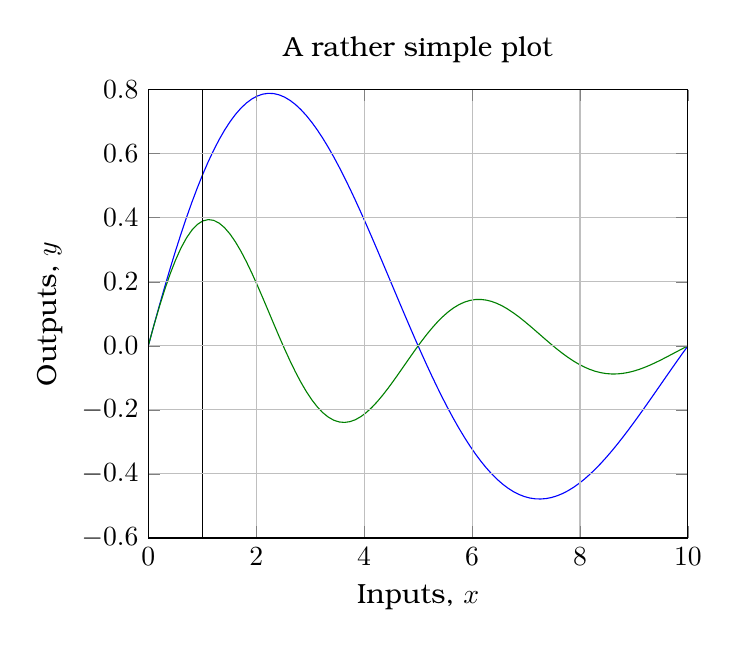
\begin{tikzpicture}

\begin{axis}[
title={A rather simple plot},
xlabel={Inputs,  $x$},
ylabel={Outputs, $y$},
xmin=0, xmax=10,
ymin=-0.6, ymax=0.8,
axis on top,
xtick={0,2,4,6,8,10},
xticklabels={$0$,$2$,$4$,$6$,$8$,$10$},
ytick={-0.8,-0.6,-0.4,-0.2,0,0.2,0.4,0.6,0.8,1},
yticklabels={,$-0.6$,$-0.4$,$-0.2$,$0.0$,$0.2$,$0.4$,$0.6$,$0.8$,},
xmajorgrids,
ymajorgrids
]
\addplot [blue]
table {%
0 0
0.101010101010101 0.0627864987208066
0.202020202020202 0.124060689746267
0.303030303030303 0.183602379292711
0.404040404040404 0.241202858356924
0.505050505050505 0.296665526060478
0.606060606060606 0.349806451039415
0.707070707070707 0.400454869823906
0.808080808080808 0.448453621431034
0.909090909090909 0.493659517670129
1.01010101010101 0.535943648932884
1.11111111111111 0.575191625508647
1.21212121212121 0.611303754728103
1.31313131313131 0.644195154494678
1.41414141414141 0.673795804011824
1.51515151515152 0.700050532754941
1.61616161616162 0.722918948968047
1.71717171717172 0.742375309186912
1.81818181818182 0.758408330501375
1.91919191919192 0.77102094746933
2.02020202020202 0.780230015782869
2.12121212121212 0.786065964962628
2.22222222222222 0.788572402519334
2.32323232323232 0.787805672170883
2.42424242424242 0.783834368839667
2.52525252525253 0.776738813276581
2.62626262626263 0.766610489266663
2.72727272727273 0.753551446464815
2.82828282828283 0.737673671989747
2.92929292929293 0.719098433969416
3.03030303030303 0.697955600281857
3.13131313131313 0.674382935772018
3.23232323232323 0.648525381247407
3.33333333333333 0.620534317563855
3.43434343434343 0.590566818107457
3.53535353535354 0.558784892959791
3.63636363636364 0.525354728002411
3.73737373737374 0.490445922171129
3.83838383838384 0.454230726015299
3.93939393939394 0.416883284647352
4.04040404040404 0.378578888089834
4.14141414141414 0.339493231935178
4.24242424242424 0.299801691134305
4.34343434343434 0.259678609619511
4.44444444444444 0.219296608348412
4.54545454545454 0.178825914228446
4.64646464646465 0.138433712247484
4.74747474747475 0.0982835229944399
4.84848484848485 0.0585346076059759
4.94949494949495 0.019341402022871
5.05050505050505 -0.0191470177173114
5.15151515151515 -0.056787437587232
5.25252525252525 -0.0934429736753208
5.35353535353535 -0.128983505057854
5.45454545454545 -0.163286070371763
5.55555555555556 -0.196235227194204
5.65656565656566 -0.227723373502972
5.75757575757576 -0.257651030663391
5.85858585858586 -0.285927087553406
5.95959595959596 -0.312469005606952
6.06060606060606 -0.33720298471895
6.16161616161616 -0.36006409011661
6.26262626262626 -0.380996340459151
6.36363636363636 -0.399952757581248
6.46464646464646 -0.416895378444016
6.56565656565657 -0.431795230000493
6.66666666666667 -0.444632267820049
6.76767676767677 -0.455395279447295
6.86868686868687 -0.464081753596032
6.96969696969697 -0.470697716395682
7.07070707070707 -0.475257536018891
7.17171717171717 -0.47778369712087
7.27272727272727 -0.47830654661634
7.37373737373737 -0.476864012406137
7.47474747474747 -0.473501296744286
7.57575757575758 -0.468270546005907
7.67676767676768 -0.461230498677594
7.77777777777778 -0.452446113444603
7.87878787878788 -0.441988179292954
7.97979797979798 -0.429932909579686
8.08080808080808 -0.416361522051021
8.18181818181818 -0.401359806806122
8.28282828282828 -0.385017684213044
8.38383838383838 -0.367428754785078
8.48484848484848 -0.348689843017847
8.58585858585859 -0.328900537171984
8.68686868686869 -0.308162726964478
8.78787878787879 -0.286580141098764
8.88888888888889 -0.264257886527864
8.98989898989899 -0.241301991299166
9.09090909090909 -0.217818952776489
9.19191919191919 -0.193915292980054
9.29292929292929 -0.169697122718245
9.39393939393939 -0.14526971611673
9.49494949494949 -0.120737097077342
9.5959595959596 -0.0962016391164428
9.6969696969697 -0.0717636799520695
9.7979797979798 -0.0475211521201942
9.8989898989899 -0.0235692308077818
10 1.44531498033966e-15
};
\addplot [green!50.0!black]
table {%
0 0
0.101010101010101 0.0620303448731334
0.202020202020202 0.120601429178462
0.303030303030303 0.174903225519708
0.404040404040404 0.224226810715517
0.505050505050505 0.267971824466442
0.606060606060606 0.305651877364052
0.707070707070707 0.336897902005912
0.808080808080808 0.361459474484024
0.909090909090909 0.379204165250687
1.01010101010101 0.390115007891434
1.11111111111111 0.394286201259667
1.21212121212121 0.391917184419833
1.31313131313131 0.383305244633331
1.41414141414141 0.368836835994873
1.51515151515152 0.348977800140929
1.61616161616162 0.324262690623703
1.71717171717172 0.295283409053728
1.81818181818182 0.262677364001205
1.91919191919192 0.227115363007649
2.02020202020202 0.189289444044917
2.12121212121212 0.149900845567153
2.22222222222222 0.109648304174206
2.32323232323232 0.069216856123742
2.42424242424242 0.0292673038029879
2.52525252525253 -0.00957350885865572
2.62626262626263 -0.0467214868376604
2.72727272727273 -0.0816430351858816
2.82828282828283 -0.113861686751486
2.92929292929293 -0.142963543776703
3.03030303030303 -0.168601492359475
3.13131313131313 -0.190498170229575
3.23232323232323 -0.208447689222008
3.33333333333333 -0.222316133910025
3.43434343434343 -0.232040876798016
3.53535353535354 -0.237628768009446
3.63636363636364 -0.23915327330817
3.73737373737374 -0.236750648372143
3.83838383838384 -0.230615249338797
3.93939393939394 -0.220994089646477
4.04040404040404 -0.20818076102551
4.14141414141414 -0.192508842106522
4.24242424242424 -0.174344921508924
4.34343434343434 -0.154081363482239
4.44444444444444 -0.132128943263932
4.54545454545454 -0.108909476388245
4.64646464646465 -0.0848485613591223
4.74747474747475 -0.0603685485386712
4.84848484848485 -0.0358818399760347
4.94949494949495 -0.0117846154038909
5.05050505050505 0.0115489310312406
5.15151515151515 0.0337717703459742
5.25252525252525 0.0545685739709792
5.35353535353535 0.073659556862599
5.45454545454545 0.090803593744708
5.55555555555556 0.105800586879304
5.65656565656566 0.118493076720424
5.75757575757576 0.128767099390827
5.85858585858586 0.136552306941577
5.95959595959596 0.141821377643245
6.06060606060606 0.14458875395717
6.16161616161616 0.144908755214958
6.26262626262626 0.142873120282179
6.36363636363636 0.138608042509705
6.46464646464646 0.132270765017966
6.56565656565657 0.124045808773686
6.66666666666667 0.114140908986544
6.76767676767677 0.102782737078552
6.86868686868687 0.0902124858865711
6.96969696969697 0.0766813948948995
7.07070707070707 0.0624462902228938
7.17171717171717 0.0477652108955134
7.27272727272727 0.0328931886966724
7.37373737373737 0.0180782437577771
7.47474747474747 0.00355765208382255
7.57575757575758 -0.0104454654025625
7.67676767676768 -0.023725189880497
7.77777777777778 -0.0360954528591778
7.87878787878788 -0.0473922585888476
7.97979797979798 -0.0574754615830318
8.08080808080808 -0.0662300881290015
8.18181818181818 -0.0735671984769764
8.28282828282828 -0.079424293956532
8.38383838383838 -0.0837652804575967
8.48484848484848 -0.0865800064341554
8.58585858585859 -0.0878833997488278
8.68686868686869 -0.0877142331993711
8.78787878787879 -0.08613355339085
8.88888888888889 -0.0832228116870949
8.98989898989899 -0.0790817392586963
9.09090909090909 -0.0738260107182608
9.19191919191919 -0.0675847424903266
9.29292929292929 -0.0604978729079194
9.39393939393939 -0.0527134710791167
9.49494949494949 -0.0443850208563396
9.5959595959596 -0.0356687248080637
9.6969696969697 -0.0267208709920781
9.7979797979798 -0.0176953026189744
9.8989898989899 -0.00874102744289201
10 5.31701667284069e-16
};
\path [draw=black, fill opacity=0] (axis cs:0,1)
--(axis cs:10,1);

\path [draw=black, fill opacity=0] (axis cs:1,-0.6)
--(axis cs:1,0.8);

\path [draw=black, fill opacity=0] (axis cs:0,0)
--(axis cs:10,0);

\path [draw=black, fill opacity=0] (axis cs:0,-0.6)
--(axis cs:0,0.8);

\end{axis}

\end{tikzpicture}
\end{center}
\blabla{1}

\subsection{Tikz}

\blabla{1}
\begin{center}
% PGF OPTIONS
\pgfplotsset{
             major grid style = {dashed, black},
             axis line style  = {black, line width = 1pt}                       
             }
% PLOT
\begin{tikzpicture}
  \begin{axis}
    [
    grid   = major,
    xlabel = {Inputs,  $x$},
    ylabel = {Outputs, $y$}, 
    title  = {A rather simple plot},
    width  = 90mm,
    height = 65mm,
    xmin = 0.,
    xmax = 10.,
    ymin = -.6,
    ymax = .8,
    %enlarge x limits = false,
    every x tick/.style = {color = black, thick},    
    ytick  = {-.6, -.4, -.2, 0., .2, .4, .6, .8},
    %enlarge y limits = false,
    every y tick/.style = {color = black, thick},        
    ]
    \addplot  [
              color      = blue,
              mark       = none,
              line width = 1pt
              ] 
             table [x index=0,y index=1,col sep=space] {simple_plot/data.csv};
    \addplot  [
              color      = teal,
              mark       = none,
              line width = 1pt
              ]
              table [x index=0,y index=2,col sep=space] {simple_plot/data.csv};
  \end{axis}
\end{tikzpicture}
\end{center}
\blabla{1}

\newpage

\section{Flo : Matlab}

\subsection{Matlab + PDF backend}
\begin{center}
\includegraphics{simple_plot/figure_matlab.pdf}
\end{center}

\subsection{Matlab + export \_fig package + PDF backend}
\begin{center}
\includegraphics{simple_plot/figure_matlab_export_fig.pdf}
\end{center}

\subsection{Matlab + matlab2tikz package}
\begin{center}
\input{simple_plot/figure_matlab_matlab2tikz.tex}
\end{center}

\subsection{Matlab2tikz + grid adjust}
\begin{center}
\input{simple_plot/figure_matlab_matlab2tikz2.tex}
\end{center}

\subsection{Subplot Matlab + matlab2tikz package}
\begin{center}
\input{simple_plot/figure_subplot_matlab2tikz.tex}
\end{center}

\subsection{Subplot Matlab + matlab2tikz + grid adjust}
\begin{center}
\input{simple_plot/figure_subplot_matlab2tikz2.tex}
\end{center}

\end{document}